%%%%%%%%%%%%%%%%%%%%%%%%%%%%%%%%%%%%%%%%%%%%%%%%%%%
%                                                 %
%                     SECTION                     %
%                                                 %
%%%%%%%%%%%%%%%%%%%%%%%%%%%%%%%%%%%%%%%%%%%%%%%%%%%

\section*{Details}

Supporting this \textit{report} the \hyperlink{https://github.com/MIMBCD-UI/testing-guide-breast/tree/master/samples/test_3}{Testing Guide} has a description of what are our goals and achievements with this \hyperlink{https://www.nngroup.com/articles/pilot-testing/}{pilot tests} phase. The tests where made by using the \hyperlink{https://github.com/MIMBCD-UI/prototype-breast-screening/releases/tag/v1.0.6-alpha}{v1.0.6-alpha} version, a pre-release version preparing our beta tests in production. The results can be accessed by this \hyperlink{https://docs.google.com/spreadsheets/d/1WwbvDO5Iz39Jr6H2ZzPth1o9DqhmpQz10Vtao7rvjfQ/edit?usp=sharing}{spreadsheet} and the raw video data is allocated in our \hyperlink{https://ulisboa-my.sharepoint.com/:f:/g/personal/francisco_calisto_office365_ulisboa_pt/EvTuVe-jyClHgNYUvCXJ1YYBUIYAKlFdjOwCDU1X5F71Kw?e=9IC0Dy}{cloud}.

\hfill

%%%%%%%%%%%%%%%%%%%%%%%%%%%%%%%%%%%%%%%%%%%%%%%%%%%

List of interviewed physicians:

%%%%%%%%%%%%%%%%%%%%%%%%%%%%%%%%%%%%%%%%%%%%%%%%%%%

\hfill

\begin{enumerate}
\item Doctor Maria Clara Aleluia;
\item Doctor Gisela Andrade;
\item Doctor Pedro Tom\'{a}s Marques;
\item Doctor Ana Sofia Costa;
\end{enumerate}

\hfill

%%%%%%%%%%%%%%%%%%%%%%%%%%%%%%%%%%%%%%%%%%%%%%%%%%%

We start the tests by using our protocol and by following the \hyperlink{https://github.com/MIMBCD-UI/testing-guide-breast/tree/master/samples/test_3}{Testing Guide}. We ask the Radiologists to do simple and clear \textit{tasks} so that they can quickly understand what is to be done. We use the \textit{think-aloud} protocol to understand the Radiologist's thinking as they are performing the set of \textit{tasks}.

\clearpage

Starting the tests with Doctor Maria Clara Aleluia, the first relevant question she asks was \textit{"Is it to use the mouse and keyboard, or we have any kind of other interaction?"}. This question is the reflex of the use of past touch-screen \cite{Calisto:2017:TTM:3132272.3134111} interactions on an early study. The Radiologist can configure the medical image freely. For the \textbf{Freehand} \textit{task}, the first participant addressed the issue of the not that clear metaphor of the icon button. She said \textit{"I thought the button was a share button and I did not press there because of that"}. Then the Doctor asks \textit{"What is better for the machine? Should we give more annotations or less?"}, where we answer that it depends. We will need to balance the \textbf{Meta-Information Generation (Info. Gen.)}.

The first participant assigns a potential issue regarding the micro-calcifications, where it would be easier to annotate the micro-calcifications by the use of a similar tool like \textbf{Freehand} for a \textbf{ROI} area. Then we ask \textit{What are the standards that will typically justify the surgery regarding the micro-calcifications?}. We have two types of patterns (Figure \ref{fig:mc_form}), on the one hand the distribution in the breast, with several forms of micro-calcifications \cite{bassett1992mammographic, shen1994application, yu2000cad} that are distributed in the breast and the most suspicious ones can be formless, that is, dispersed or grouped. In clusters, those that are distributed in a linear form towards the nipple are the most suspect. However, micro-calcifications itself have different morphologies: (i) they may be rounded; (ii) may be of the "grain of salt" type in a similar form; (iii) may be irregular as if they were "commas"; and (iv) may also appear to be a "tile", these being the most severe.

%%%%%%%%%%%%%%%%%%%%%%%%%%%%%%%%%%%%%%%%%%%%%%%%%%%

\hfill

\begin{figure}[h]
\centering
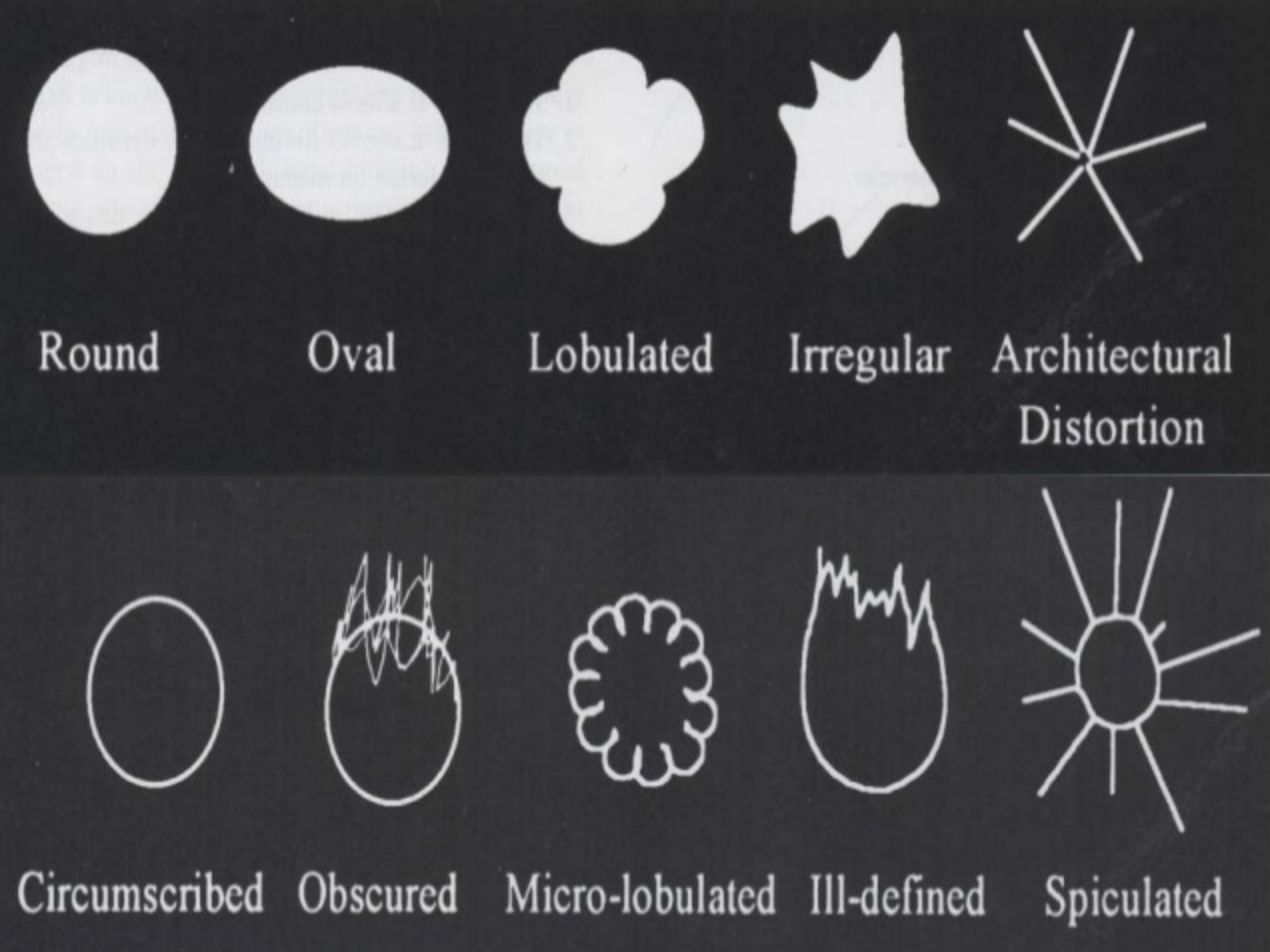
\includegraphics[width=\textwidth]{mc_form}
\caption{Form of the Micro-Calcifications.}
\label{fig:mc_form}
\end{figure}

\hfill

%%%%%%%%%%%%%%%%%%%%%%%%%%%%%%%%%%%%%%%%%%%%%%%%%%%

Therefore, the distribution \cite{berg2002does, chan1987image} is another variable, if it is distributed (Figure \ref{fig:mc_dist}) in triangle pointing to the nipple is quite severe. On the other hand, if it is in the form of a rectangle, it will not be so severe. Finally, there is a dependence on the morphology of micro-calcifications, however this morphology is quite difficult to obtain. The second \textit{task} did not show any important information to be reported. Finally on the third \textit{task}, the Doctor report that the annotated task was not a lesion. It was not a problem at first, since we are just testing interaction and not knowledge over the domain.

%%%%%%%%%%%%%%%%%%%%%%%%%%%%%%%%%%%%%%%%%%%%%%%%%%%

\hfill

\begin{figure}[h]
\centering
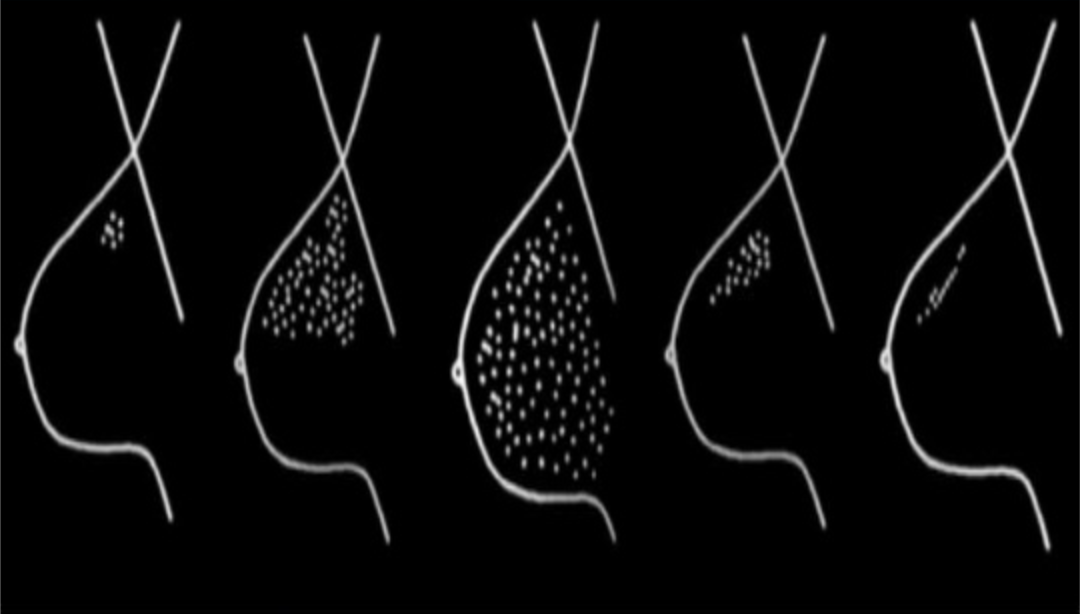
\includegraphics[width=\textwidth]{mc_dist}
\caption{Distribution of the Micro-Calcifications.}
\label{fig:mc_dist}
\end{figure}

\hfill

%%%%%%%%%%%%%%%%%%%%%%%%%%%%%%%%%%%%%%%%%%%%%%%%%%%

For the second participant, Doctor Gisela Andrade, she start with some doubts related with the \textit{task}. She did not understood at first the information on the table. One of the misunderstood was the fact that the date was in a different form. The Doctor show little confidence, but it seems to be the Doctor profile. Finally, for the last question the Doctor understood the need to close the last patient to open a new one. The Doctor is not using the \textbf{Zoom} feature.

\clearpage

The third participant, Doctor Pedro Tom\'{a}s Marques, start with some delay on understanding how to start, but quickly understood. We first address an error related with the fact that each time the user does a click it also do the \textit{Zoom} feature. We also underline the fact that the participant need to save, however, the participant always remember to save the annotation. For the next task, the participant try to explore a little bit more of the \textbf{Toolbar}. At the third \textit{task}, the participant quickly understood the \textit{task} and annotate the lesion that is not a real lesion, but was considered so. The participant used the \textbf{Zoom}, \textbf{Invert} and the \textbf{WW/WC} features to manipulate the image and respective frame. Despite of the performance of this participant, several \textit{System Error} occurred at minute 5:20, that where not the participant's fault, but need to be reported and \hyperlink{https://github.com/MIMBCD-UI/prototype-breast-screening/issues}{GitHub issues} were created.

Last but not least, the fourth participant, Doctor Ana Sofia Costa, start the \textit{tasks} normally. This participant did not report anything relevant since she was observing the previous tests, the tests from Doctor Pedro Tom\'{a}s Marques. The participant was really sensitive to the annotations of the first \textit{task}. A high number of annotations was done. And the annotations were closed (Figure \ref{fig:error}) during the process and more or less in the middle of the annotation process, so that the participant simulates the continuation of them. The second \textit{task}, was not underlined the need to save. The participant saved anyway. Finally, for the last \textit{task} the participant showed confidence and quickly annotate the lesion. However, the participant argue that it should be interesting a more easy way to \textbf{Zoom} during the annotation process.

%%%%%%%%%%%%%%%%%%%%%%%%%%%%%%%%%%%%%%%%%%%%%%%%%%%

\hfill

\begin{figure}[h]
\centering
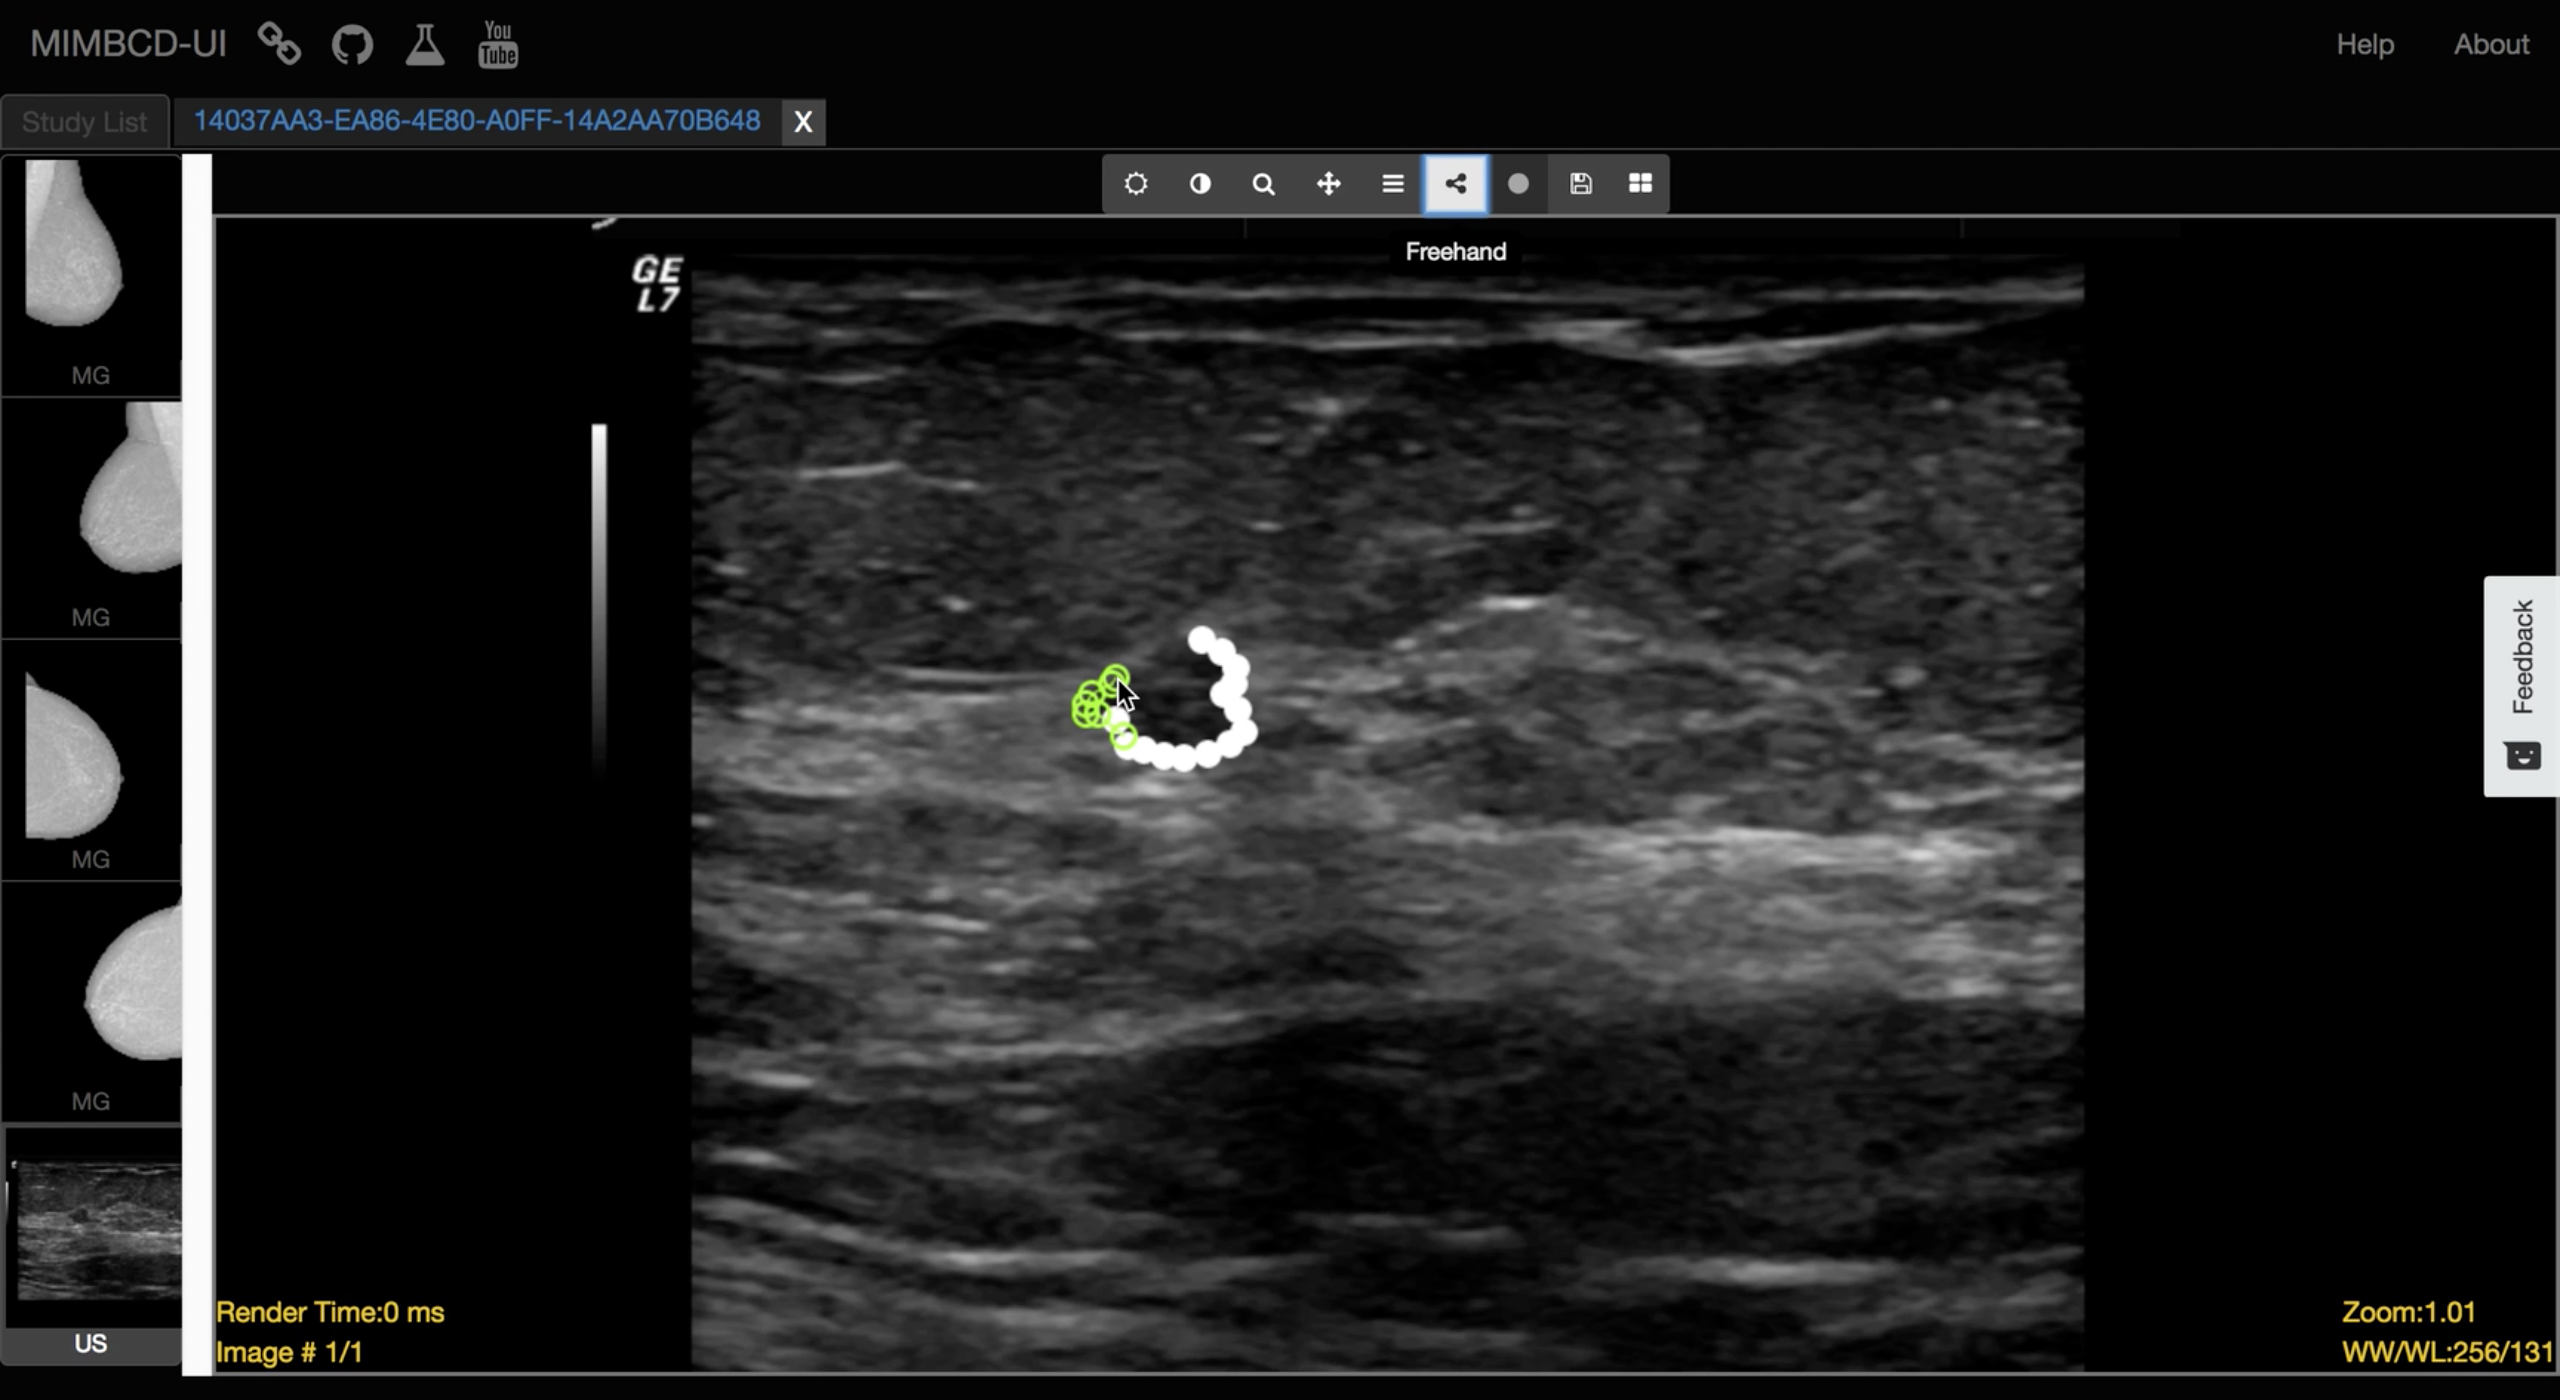
\includegraphics[width=\textwidth]{error}
\caption{Annotation Error during the annotation process at the second \textit{task} of the participant number four.}
\label{fig:error}
\end{figure}

\hfill

%%%%%%%%%%%%%%%%%%%%%%%%%%%%%%%%%%%%%%%%%%%%%%%%%%%

At the end we gratefully say thanks for the user study of the \hyperlink{https://www.nngroup.com/articles/pilot-testing/}{pilot tests}. And the participants showed to be useful for this phase. While we just need to test a pre-release version of our system, it was of chief importance the descriptions and the issues discovered.

%%%%%%%%%%%%%%%%%%%%%%%%%%%%%%%%%%%%%%%%%%%%%%%%%%%